\section{Programmable monetary architecture, incidence and accounting}
\subsection{Sovereign architecture and the boundary of the model}
The intended long-run design is sovereign programmable payment money. To obtain a tractable first model, all transaction balances are direct sovereign liabilities. Firms finance capital formation from retained earnings, and equity is owned by households. There is no endogenous bank credit, government bond market, foreign sector or asset-price equilibrium. This is a limiting monetary architecture with fully sovereign transaction balances, not a description of the current euro area or a complete narrow-banking transition proposal.

The simplification is consequential. Moving existing deposits onto sovereign accounts requires counterpart assets, bank funding arrangements, redemption rules and a plan for legacy debts. A sovereign state does not acquire the entire stock of existing broad money as spendable revenue by relabelling it. The current EU debt stock also cannot be wished away. The empirical context includes an EU debt ratio of 81.7\% in the annual 2025 first notification \citep{eurostat2026}; that liability is deliberately outside the simulated balance sheet. Thus the simulations test a conditional post-reform monetary mechanism, not the financing of the reform itself.

\subsection{Why programmable monetary infrastructure matters for usownership}
The technological claim is not that software changes the resource constraint. It is that the administrative architecture of ownership is changing as money, securities and other claims become increasingly digital and, in some settings, tokenised. The prevailing account-based paradigm typically separates identity and contribution data, company share registers, custodians, payment systems, tax records and corporate-action processing. Each institution can work well on its own, but a recurrent grant to millions of heterogeneous participants requires repeated matching and reconciliation across those systems.

An Internet-of-Value architecture changes the implementation problem by making the asset claim and some of its transfer rules machine-readable or executable. BIS work on tokenisation and unified ledgers emphasises composability and atomic settlement between money and assets rather than a requirement for permissionless cryptocurrency \citep{bis2022,bis2023,bis2025}. The European Commission similarly describes tokenisation and DLT as a possible route toward an ``Internet of Value'' \citep{eciov2026}. In that environment, a verified contribution event can update a fractional ownership claim; vesting can be enforced at the claim layer; dividends and corporate actions can follow the current holder; and a sale or voluntary diversification can settle conditionally against digital money. The same infrastructure can automate an MVI payment, a protected transaction balance, or a monetary levy and cancellation rule. It therefore provides a common execution substrate for the \emph{ownership bridge} and the \emph{income bridge}.

\begin{figure}[htbp]\centering
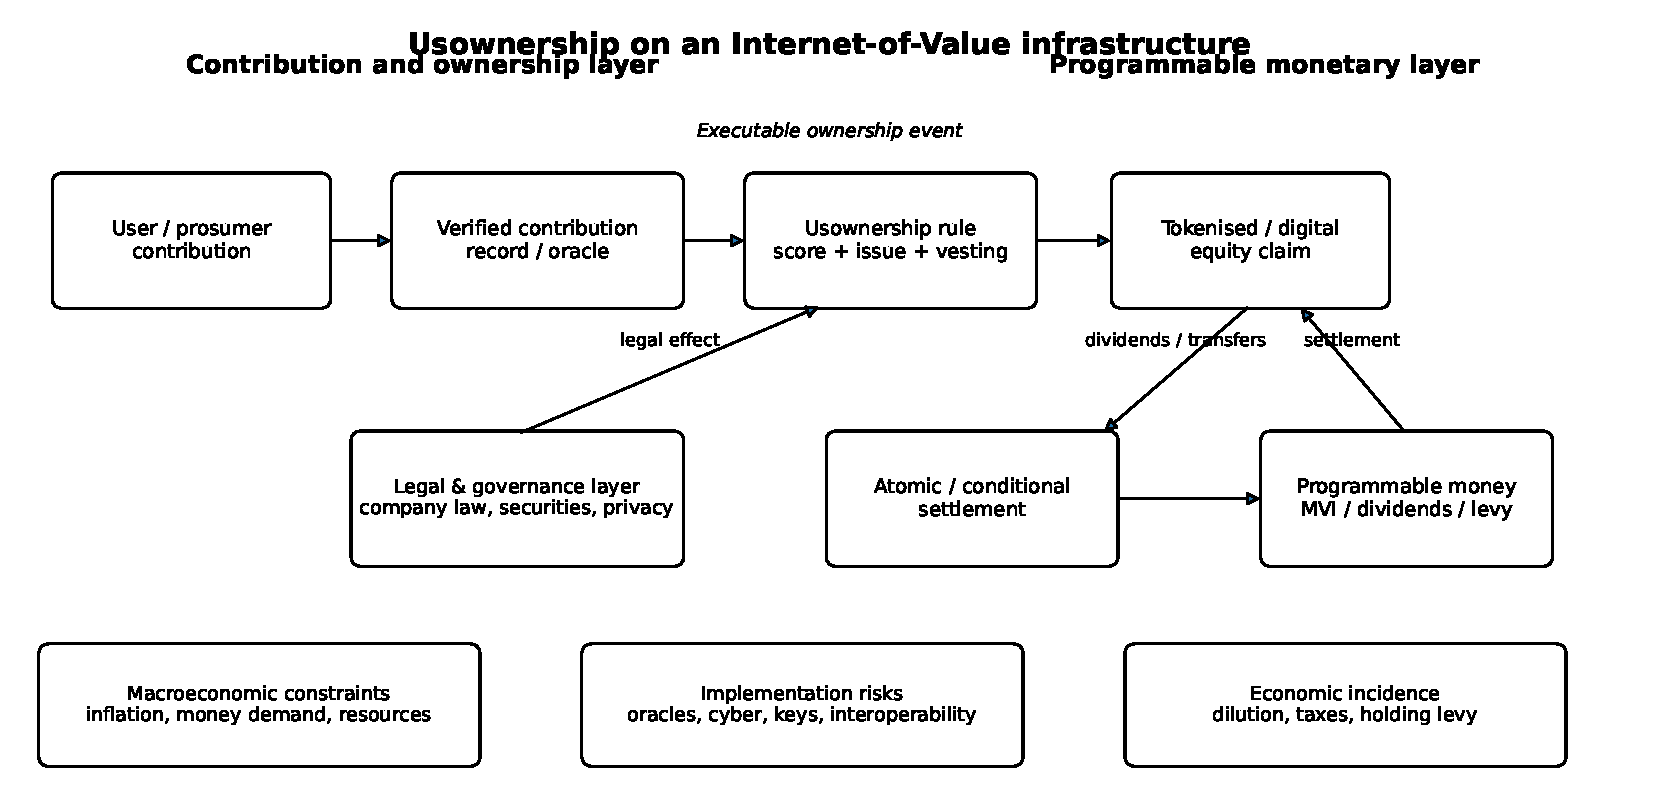
\includegraphics[width=.96\linewidth]{figures/programmable_usownership_architecture.pdf}
\caption{Usownership on programmable Internet-of-Value infrastructure. Programmability coordinates contribution evidence, equity rights and payment; legal validity, valuation, privacy and macroeconomic incidence remain outside the ledger and must be governed separately.}
\label{fig:programmable-usownership}
\end{figure}

The comparison can be stated as a measurable break-even condition rather than a technological slogan. Let $N_t$ be the number of ownership events in period $t$, $c_L$ the marginal legacy-system processing and reconciliation cost per event, $c_P$ the marginal programmable-infrastructure cost, $F_P$ its fixed operating cost, and $C_O,C_R,C_{Pr}$ the incremental costs of trustworthy contribution oracles, regulatory compliance and privacy/cybersecurity. A direct implementation advantage requires
\begin{equation}
N_t(c_L-c_P)>F_P+C_O+C_R+C_{Pr}.
\label{eq:implementation}
\end{equation}
No numerical saving is imposed in the simulation because these terms have not been empirically estimated for a national usownership regime. Equation~\eqref{eq:implementation} instead identifies the evidence required. The hypothesis becomes stronger as awards become more frequent and granular, and weaker if oracle, compliance or interoperability costs dominate the reduction in reconciliation cost.

\begin{table}[htbp]\centering\small
\caption{Implementation comparison: separate account systems and programmable value rails}
\begin{tabularx}{\linewidth}{@{}p{.22\linewidth}p{.34\linewidth}X@{}}
\toprule
Dimension & Prevailing account-based implementation & Programmable Internet-of-Value implementation \\
\midrule
Ownership record & Separate corporate/share registry and custodial records & Tokenised or digitally executable ownership claim \\
Award execution & Batch or manual reconciliation across systems & Conditional rule can update claim after verified event \\
Money/asset settlement & Payment and asset legs may use distinct infrastructures & Atomic or conditional settlement can coordinate both legs \\
Granularity & Economical for many conventional plans but micro-awards can face fixed frictions & Fractional recurrent awards can have low marginal execution cost if infrastructure is shared \\
Corporate actions & Multiple intermediaries propagate dividends, splits and transfers & Rules can propagate actions to the current claim holder \\
Policy control & Fiscal and monetary ledgers are separately administered & Issuance, protected balances, levies and burns can be auditable machine-executable rules \\
Unresolved constraints & Tax, securities, privacy, insolvency and valuation law & Same legal constraints plus oracle, cyber, key-management and interoperability risks \\
\bottomrule
\end{tabularx}

\end{table}

This framing also clarifies the word \emph{programmable}. The current digital-euro project rejects purpose-restricted ``programmable money'', while contemplating conditional payments \citep{ecbfaq2026}. Our proposal therefore concerns \emph{programmable monetary infrastructure}: rules for issuance, settlement, protected balances and cancellation can be machine-executed without restricting ordinary currency to state-approved purchases. A tokenised share is still a legal corporate claim; a smart contract cannot manufacture a valid contribution observation, determine insolvency priority by itself, or make dilution costless. Programmability is an adoption technology, not a new source of seigniorage.

Let $N_t=P_tY_t$ denote nominal GDP, $M_t$ end-of-period sovereign transaction balances, $G_t$ public purchases, $H_t$ transfers, $T_t$ conventional tax receipts and $B_t$ the monetary holding levy permanently cancelled. Define fiscal issuance before the holding levy as
\begin{equation}
F_t=G_t+H_t-T_t,\qquad M_t-M_{t-1}=F_t-B_t.\label{eq:budget}
\end{equation}
$F_t$ is a \emph{net-of-conventional-tax financing flow}, not total gross expenditure and not necessarily positive. A negative value retires currency. We report it separately from genuine net money financing $(M_t-M_{t-1})/N_t$. Counting $F_t$ and $B_t$ as independent free resources would be incorrect.

\begin{proposition}[No free monetary recycling]
Under the consolidated budget identity \eqref{eq:budget}, a currency burn can expand the expenditure financed by a given net change in money only by transferring an equal nominal amount from the balances charged. Recycling does not remove the financing incidence.
\end{proposition}
\begin{proof}
Rearranging gives $G_t+H_t=T_t+B_t+(M_t-M_{t-1})$. At a fixed net monetary change and conventional receipts, an additional unit of expenditure requires an additional unit of levy. Implementation as a fee followed by cancellation does not change the identity.
\end{proof}

With $m_t=M_t/P_t$ and $\pi_t=P_t/P_{t-1}-1$, the exact discrete decomposition is
\begin{equation}
\frac{F_t}{P_t}=m_t-m_{t-1}+\frac{\pi_t}{1+\pi_t}m_{t-1}+\frac{B_t}{P_t}.\label{eq:seign}
\end{equation}
This separates the change in real balances, the valuation effect of inflation on opening balances and the explicit holding levy. It is distinct from an operational central bank's earnings on assets net of funding and operating costs. An interest-bearing liability would require its remuneration in the budget. Broad deposit inflation losses are not automatically government revenue.

\subsection{An analytical financing envelope}
For a transparent steady-growth calculation, let the end-of-period money/GDP ratio be $k$, real growth $g$, inflation $\pi$, nominal growth $n=(1+g)(1+\pi)-1$, and a uniform annual holding levy $d$ on opening balances. Then
\begin{equation}
s_{\rm net}=\frac{k n}{1+n},\qquad b=\frac{k d}{1+n},\qquad f=\frac{k(n+d)}{1+n}.\label{eq:frontier}
\end{equation}
Here $f=F/N$ is gross fiscal financing before the holding levy and $b=B/N$ is levy incidence. None of these equals $\pi$ automatically. Illustrate endogenous monetary demand with
\begin{equation}
k(\pi,d)=k_0\exp[-\varepsilon(\pi+d)],\qquad \varepsilon>0.\label{eq:cagan}
\end{equation}
This is a behavioural specification, not an estimated elasticity or the exact liquidity rule used in the heterogeneous model.

\begin{proposition}[Finite levy-assisted financing]
Holding $g$ and $\pi$ fixed under \eqref{eq:frontier}--\eqref{eq:cagan}, the derivative of $f$ with respect to $d$ has the sign of $1-\varepsilon(n+d)$. An unconstrained interior revenue maximum is $d^*=1/\varepsilon-n$, with boundary solutions when that value lies outside the permitted levy interval.
\end{proposition}
\begin{proof}
Differentiation yields $\partial f/\partial d=k_0e^{-\varepsilon(\pi+d)}[1-\varepsilon(n+d)]/(1+n)$. The prefactor is positive. A shrinking money-demand base eventually offsets the larger charge where the turning point lies within the interval.
\end{proof}

This is a revenue maximum, not a welfare optimum. A high revenue-maximising levy can impose severe payment, distributional and substitution costs. As an illustrative calculation, $k_0=0.6$, $\varepsilon=4$, $g=3\%$, $\pi=2\%$ and $d=4\%$ imply $k\simeq0.472$ and gross capacity of about 4.07\% of GDP. About 1.80 percentage points are the explicit holding levy; only about 2.27 are net monetary finance. Even the unrestricted revenue optimum in this example is not a source of resources remotely equivalent to half of GDP.

A rise in real productive capacity can increase desired money balances or accommodate higher nominal spending, but it does not create an unconditional right to issue a matching amount. Under $MV=PY$, $\Delta\log P=\Delta\log M+\Delta\log V-\Delta\log Y$ is an identity. Predicting inflation additionally requires behaviour and a price/output closure. Our simulation supplies such a closure explicitly instead of treating this identity as a forecasting equation.

\begin{figure}[htbp]\centering
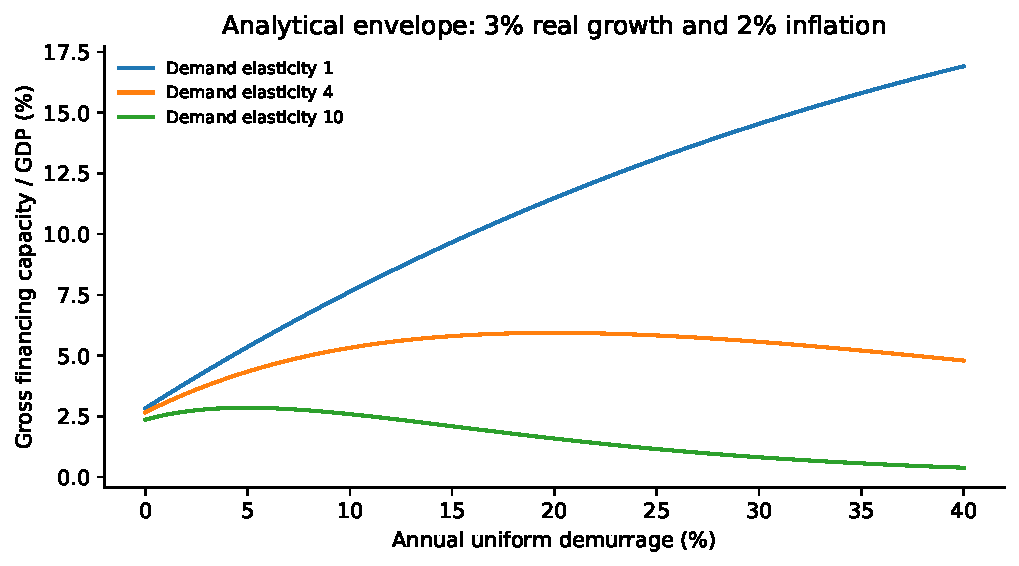
\includegraphics[width=.92\linewidth]{figures/frontier.pdf}
\caption{Analytical gross financing envelope with endogenous money demand. Values are assumed scenarios, not observed national revenue capacities. The holding levy is part of the resource transfer.}
\end{figure}

